\chapter{Transformadores de protección}
\section{Transformadores de medida y protección}
\subsection{Funciones básicas}
\begin{itemize}
	\item Adaptar las señales de alta intensidad y tensión de primario a valores secundarios estandarizados
	\item Aislar la parte de baja tensión de la de alta tensión para la medida
\end{itemize}
\subsection{Características generales}
\begin{itemize}
	\item En el secundario magnitud proporcional a la del primario
	\item El primario con aislamiento correspondiente a la red AT
	\item El primario y el secundario muy bien aislados entre sí
	\item El secundario se conecta siempre a tierra
	\item Debe comprobarse que la saturación con $I_k$ no afecta a la seguridad
	\item Deben soportar los efectos térmicos y dinámicos de las sobreintensidadesmáximasen el punto de instalación
	\item Deben soportar sobretensionesde maniobra, puesta a tierra accidental de una fase y atmosféricas
	\item Medidas de protección para el caso de explosión de los transformadores
	\item Todas las partes metálicas que no estén sometidas a tensión deben ponerse a tierra
	\item Debe conectarse a tierra el secundario (o separarse del primario mediante pantallas puestas a tierra)
	\item Transformadores de intensidad: debe permitir la desconexión de los aparatos alimentados sin interrumpir la continuidad del secundario
	\item Transformadores de medida: dimensionado de los conductores del secundario para que no se sobrepase la carga de precisión ni una caída de tensión del 1\%
\end{itemize}
\subsection{Tipos}
\begin{itemize}
	\item Transformadores de intensidad
	\begin{equation}
		I_s=1A \ o \ 5A
	\end{equation}
	\begin{itemize}
		\item Para la potencia de diseño prevista la intensidad secundaria esté entre el 45 \%(20 \% para clase 0,2S ó 0,5 S) de la intensidad asignada y el 100 \% de la intensidad térmica permanente asignada al transformador
	\end{itemize}
	\item Transformadores de tensión
	\begin{equation}
		U_s=100V \ o \ 110V
	\end{equation}
	\begin{itemize}
		\item Tensión asignada del primario comprendida entre el 100 \% y 120 \% de la tensión nominal del circuito de potencia primario
	\end{itemize}
\end{itemize}

\section{Trasformadores de Intensidad TIs}
\subsection{Características funcionales y constructivas}
\begin{figure}[H]
	\centering
	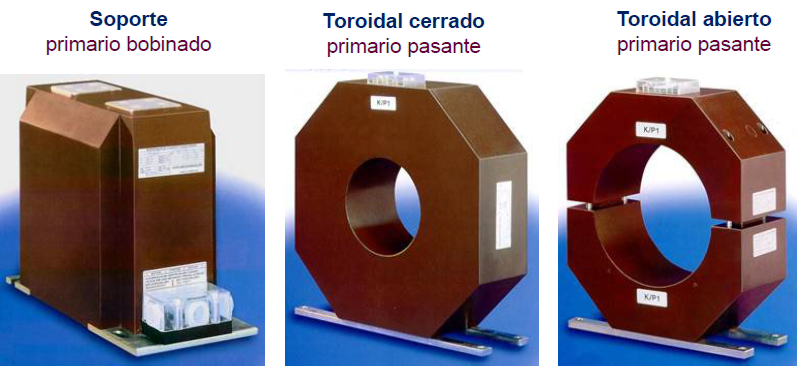
\includegraphics[width=0.7\linewidth]{Images/47}
	\label{fig:47}
\end{figure}

Ventajas del primario bobinado:
\begin{itemize}
	\item Permite mayor potencia de precisión
	\item Permite trabajar con corrientes de primario más bajas
\end{itemize}
\subsection{Comparación transformadores de potencia y de intensidad}
\begin{table}[H]
	\centering
	\begin{tabular}{|p{5cm}|p{5cm}|}
		\hline
		\textbf{Potencia} & \textbf{Intensidad} \\ \hline
		Tensión primario constante & Tensión primario no constante: caída de tensión\\ \hline
		  Cambio de $Z_S$ $\Rightarrow$ Cambio de $I_P$ & $Z_S$ y $I_P$ son independientes\\ \hline
		  IS causa – IP efecto& IP causa – IS efecto\\ \hline
		\textbf{Objetivo:} cambio del valor de tensiones e intensidades & \textbf{Objetivo:} proporcionalidad entre intensidades \\ \hline
	\end{tabular}
	\label{tab:potencia_intensidad}
\end{table}
\subsection{Cuestiones básicas de operación}
\begin{itemize}
	\item El primario está en serie con el circuito principal
	\item El secundario prácticamente en cortocircuito, \textbf{Nunca en abierto} porque explota. No debe protegerse el secundario con fusibles ni interruptores automáticos. Antes de desconectar la carga debe cortocircuitarse el secundario. 
\end{itemize}
\subsection{Características técnicas}
\begin{itemize}
	\item \textbf{Intensidad primaria asignada $I_{pn}$}: Valores normalizados (A) con sus múltiplos y submúltiplos. 10 – 12,5 – 15 – 20 – 25 – 30 – 40 – 50 – 60 – 75
	\item \textbf{Intensidad secundaria asignada $I_{sn}$}: Valores normalizados (A). 1 - 2 - 5
	\item \textbf{Relación de transformación nominal $k_n$}
	\begin{equation}
		k_n=\dfrac{I_{pn}}{I_{sn}}
	\end{equation}
	\item \textbf{Error de relación o error de intensidad $\varepsilon_i(\%)$}
	\begin{equation}
		\varepsilon_i=\dfrac{k_n\cdot I_s-I_p}{I_p}
	\end{equation}
	\item \textbf{Error de fase, desfase, o error de ángulo $\delta_i$}
	\begin{equation}
		\delta_i=\varphi_{is}-\varphi_{ip}
	\end{equation}
	\item \textbf{Error compuesto $\varepsilon_c$}
	\begin{equation}
		\varepsilon_c=\dfrac{100}{I_p}\cdot\sqrt{\dfrac{1}{T}\int_0^T\left(k_n\cdot i_s - i_p\right)\, dt}
	\end{equation}
	\item \textbf{Carga de precisión o carga nominal $Z_p$}
	\item \textbf{Potencia de precisión o potencia nominal $S_n$}: Valor de la potencia aparente, referida a la intensidad asignada, para la que se especifican los errores de relación y de ángulo.
	\begin{equation}
		S_n=Z_p\cdot I_{sn}^2
	\end{equation}
	\item \textbf{Intensidad térmica de cortocircuito asignada $I_{th}$}: Valor eficaz de la intensidad primaria máxima que el transformador soporta durante 1 segundo con el secundario en cortocircuito, sin sufrir efectos perjudiciales
	\item \textbf{Intensidad dinámica asignada $I_{dyn}$}: Valor de cresta que el transformador debe soportar con el secundario en cortocircuito, sin sufrir efectos perjudiciales
	\begin{equation}
		I_{dyn}=2.5I_{th}
	\end{equation}
	\item \textbf{Intensidad térmica permanente asignada o intensidad de calentamiento}: Valor máximo de la corriente primaria, con el secundario conectado a la carga de precisión, sin que el calentamiento sea excesivo. 	Salvo indicación expresa del fabricante, la intensidad de calentamiento es igual a la intensidad primaria asignada
	\item \textbf{Trafo de medida}
	\begin{itemize}
		\item \textbf{Clase de precisión de TI de medida}: Límite del error de relación en \% para la intensidad nominal del primario con la carga del secundario igual a la de precisión, $Z_p$.
		\begin{itemize}
			\item Clase 0,1 – Laboratorio
			\item Clase 0,2 – Laboratorio, patrones portátiles y contadores de precisión
			\item Clase 0,5 – Contadores normales, aparatos de medida
			\item Clase 1 – Aparatos de cuadro
			\item Clase 3 – Usos que no se requiera una mayor precisión
			 
		\end{itemize}
		\item \textbf{Intensidad primaria límite asignada}: Intensidad primaria mínima para la cueal el $\varepsilon_c \ge 10\%$ con $Z_p$
		\item \textbf{Factor de seguridad FS}: Relación entre la intensidad primaria límiteasignada y la intensidad primaria asignada. Expresa la saturación a través del múltiplo de la $I_{pn}$ para la que $\varepsilon_i$ tiene un valor mínimo. El valor habitual exigido para FS es 5 que significa:
		\begin{equation}
			5\cdot I_{pn}  \rightarrow \varepsilon_i \le -10\%
		\end{equation}
	\end{itemize}
	\item \textbf{Trafo de protección}
	\begin{itemize}
		\item \textbf{Intensidad primaria límite de precisión asignada $ I_{p-max-a}$}:  Intensidad primaria máxima para la cual el $\varepsilon_c$ debe cumplir las especificaciones
		\item \textbf{Clase de precisión de TI de protección } Límite del error compuesto en \% para la intensidad límite de precisión con la carga de precisión $Z_p$ Se indica antes de la P. Ejemplos: 5P 10P
		\item \textbf{Factor límite de precisión nominal $FLP_n$} Relación entre la intensidad primaria límite de precisión asignada y la intensidad primaria asignada para la que se mantiene la clase de precisión. Valores normalizados: 5, 10, 15, 20 y 30. Se indica a continuación de la P. Ejemplos: 5P10 5P20
		\item \textbf{Factor límite de precisión actual $FLP_a$}: Relación entre la intensidad primaria límite de precisión actua $ I_{p-max-a}$ y la intensidad primaria asignada. Tiene en cuenta que la influencia de la carga en la precisión es proporcional la relación entre la carga de precisión y la carga actual del TI.
		\begin{equation}
			FLP_a=FLP_n\dfrac{S_{internaTI}+S_{precisiónTI}}{S_{internaTI}+S_{actual2TI}}
		\end{equation}
		\begin{equation}
			I_{p-max-a}=FLP_a\cdot I_{pn}
		\end{equation}
		Para que se mantenga la precisión:
		$I_{kmax}< I_{p-max-a}$
	\end{itemize}
\end{itemize}
\subsubsection{Tensión inducida en el secundario}
Sea el circuito del secundario el siguiente:
\begin{figure}[H]
	\centering
	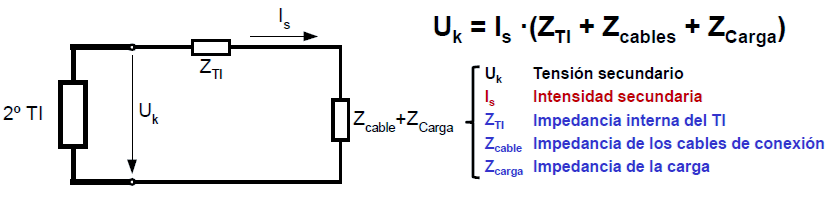
\includegraphics[width=0.7\linewidth]{Images/48}
	\label{fig:48}
\end{figure}

La tensión de saturación del TI, $U_k'$
\begin{equation}
	U_k'=FLP\cdot I_{sn}\cdot \left(Z_{TI}+Z_p\right)
\end{equation}
Se mantienen la precisión siempre que:
\begin{equation}
	U_k<U_k'
\end{equation}
\subsubsection{Clases de protección de transformadores de intensidad}
\begin{itemize}
	\item \textbf{Clase P}: TI para protección sin límite de flujo remanente y para el que se específica la saturación en caso de cortocircuito simétrico.
	\begin{itemize}
		\item Clase PR:con límite de flujo remanente. Deben asegurar la protección como un factor de remanencia (relación entre flujo remanente y el flujo de saturación) limitado para los que, en algunos casos, puede especificarse un valor de la constante de tiempo del bucle secundario y/o un valor máximo de la R del secundario. 
		\item Clase PX: baja reactancia de dispersión (sin entrehierros)
		\item Clase PXR: mismas prestaciones que PX pero con entrehierros para evitar la saturación producida por componentes de corriente continua
	\end{itemize}
\end{itemize}
\begin{table}[H]
	\centering
	\begin{tabular}{|p{3cm}|p{3cm}|p{3cm}|}
		\hline
		\textbf{Clase de precisión} & \textbf{Error de intensidad para la intensidad primaria asignada en \%} &  \textbf{Error compuesto para la intensidad límite de precisión en \%} \\ \hline
		5P y 5PR & $\pm 1$ & 5 \\ \hline
		10P y 10PR & $\pm 3$ & 10 \\ \hline
	\end{tabular}
	\caption{Carga con factor de potencia entre 0,8 inductivo y la unidad}
	\label{tab:precision}
\end{table}
\begin{table}[H]
	\centering
	\begin{tabular}{|c|p{10cm}|}
		\hline
		\textbf{Clase de precisión} & \textbf{Usos generalizados} \\ \hline
		5P & Relés diferenciales, de distancia, direccionales, de contacto a tierra y otros de cierta precisión. En general, todos aquéllos a los que afecte el error de ángulo. \\ \hline
		10P & Relés ordinarios de protección y otros. En general, aquéllos a los que no afecte el error de ángulo. \\ \hline
	\end{tabular}
	\label{tab:usos_precision}
\end{table}
Se escribe: \textit{Clase de precisión} - P - \textit{Factor límite de precisión}


\subsection{Clases TP: respuesta en régimen transitorio}
\begin{itemize}
	\item TPX núcleo sin entrehierros pero de sección suficiente como para responder al transitorio. Refleja bien la componente aperiódica. 
	\item TPY pequeños entrehierros en el núcleo para reducir la inducción remanente. Refleja bien la componente aperiódica.
	\item TPZ entrehierros superiores al TPY. Refleja bien la componente alterna,pero no a la periódica. Debido a los entrehierros no es posible obtener mucha precisión con $I_n$
\end{itemize}

Para seleccionar el tipo de TP hay que tener en cuenta:
\begin{itemize}
	\item Constante de tiempo de la línea
	\item Características del cortocircuito
	\item Precisión necesaria a intensidad nominal
	\item Precisión necesaria durante el transitorio
\end{itemize}


\subsection{Esquemas de conexión}
Existen distintas conexiones en función de la cantidad de tomas intermedias de los transformadores. No obstante, existen varias formas de medida de corriente en un sistema trifásico.
\begin{figure}[H]
	\centering
	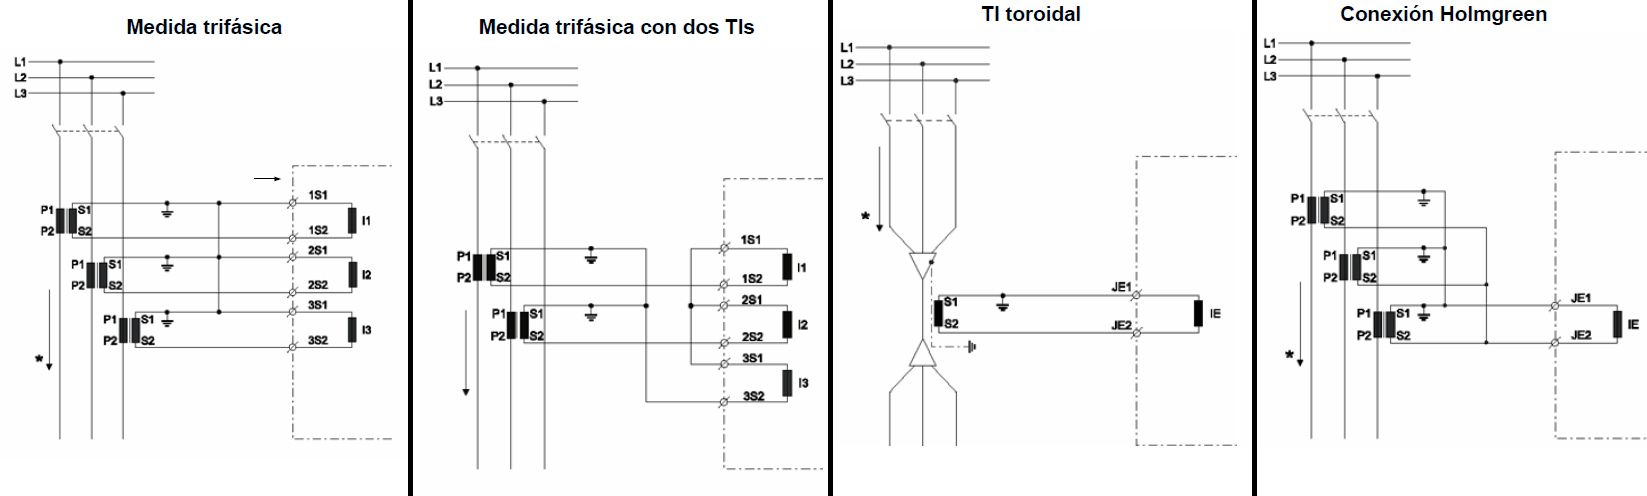
\includegraphics[width=1\linewidth]{Images/49}
	\label{fig:49}
\end{figure}
\subsection{Ejemplo de selección}
Se elige la intensidad nominal de tal forma que aguante 2 veces la intensidad nominal del trafo:
\begin{equation}
	I_{pn}=2\times\dfrac{S_n}{\sqrt{3}U_1}
\end{equation}
La intensidad nominal asignada se elige la de 5A
\begin{equation}
	I_{sn}=5A \rightarrow r_{tI}=\dfrac{I_{pn}}{I_{sn}}
\end{equation}
Se calcula la carga conectada al secundario $R_{carga}$ y su potencia
\begin{equation}
	S_{carga}=R_{carga}\cdot I^2_{sn} < S_{pTI}
\end{equation}
Se elige la clase de precisión en función de la importancia de protección. Normalmente \textbf{5P}.
\newline
Para calcular el $FLP$ y $S_{nTI}$ se calculan las intensidades máximas:
\begin{equation}
	I_{k1max}=\dfrac{S_{cc}}{\sqrt{3}U_1}\rightarrow I_{k2max}=\dfrac{I_{k1max}}{r_{tI}} \rightarrow U_k=I_{k2max}\cdot (R_{carga} +R_{TI})
\end{equation}
La tensión de saturación máxima:
\begin{equation}
	U_k'=FLP_n\cdot I_{sn} \cdot \left(R_{TI}+\dfrac{S_{pTI}}{I_{sn}^2}\right)
\end{equation}
Se selecciona un trafo:
\begin{itemize}
	\item Seleccionar factor límite de precisión $FLP_n$: Se puede seleccionar como la relación entre la intensidad de cortocircuito máxima y la intensidad primaria nominal:
	\begin{equation}
		FLP_a> \dfrac{I_{k1max}}{I_{pn}} \xrightarrow{\textbf{Si la carga es la nominal}} FLP_n> \dfrac{I_{k1max}}{I_{pn}}
	\end{equation}
	\item Seleccionar potencia de precisión $S_{pTI}$
	\item Seleccionar resistencia de devanado $R_{TI} $
\end{itemize}
Se comprueba que:
\begin{equation}
	U_k< U_k'
\end{equation}
\begin{equation}
	S_{pTI}>S_{carga}
\end{equation}
Se selecciona el factor de precisión actual:
\begin{equation}
	FLP_a=FLP_n\dfrac{R_{TI}\cdot I^2_{sn}+S_{pTI}}{R_{TI}\cdot I^2_{sn}+S_{carga}}
\end{equation}
\begin{equation}
	I_{p-max-a}=FLP_a\cdot I_{pn}
\end{equation}
Se comprueba que el TI no satura durante el cortocircuito máximo:
\begin{equation}
	I_{k1max}<I_{p-max-a}
\end{equation}
Se calcula la intensidad térmica de cortocircuito a partir del tiempo de actuación de las protecciones, $ t_{prot}$ y se elige la superior:
\begin{equation}
	I^2_{th}\cdot 1 = I_{k1max}^2\cdot t_{prot}
\end{equation}
La intensidad dinámica asignada se elige como:
\begin{equation}
	I_{dyn}>2.5\cdot I_{th}
\end{equation}
\section{Transformadores de tensión TTs}
\subsection{Características funcionales y constructivas}
\begin{itemize}
	\item Se utilizan para alimentar bobinas voltimétricas
	\item La constitución y forma de trabajo de los de tipo inductivo es como los transformadores de potencia
	\item Pueden ser inductivos o capacitivos (acoplo de la alta frecuencia, unipolar conexión fase-tierra, a partir de 66kV).
\end{itemize}

Cuestiones básicas de funcionamiento:
\begin{itemize}
	\item Tensión secundaria proporcional a tensión primaria
	\item Desfase próximo a cero
	\item Pequeña potencia secundaria
	\item Protección secundaria con fusibles
	\item Secundario puesto a tierra
\end{itemize}


\subsection{Características técnicas}
\begin{itemize}
	\item \textbf{Tensión primaria asignada $U_{pn}$} Valores normalizados kV, Debe estar entre el 100 \% y el 120 \% de la tensión nominal de la red:
	\newline
	1,1 – 2,2 – 3,3 – 5,5 – 6,6 – 11 – 13,2 – 16,5 – 22 – 27,5 – 33 – 44 – 55 – 66 kV
	\item \textbf{Tensión secundaria asignada $U_{sn}$} 
	\newline
	Conectado entre fases: 110 V (preferentemente) o 100 V
	\newline
	Conectado entre fase-tierra: $\dfrac{110}{\sqrt{3}}$ V (preferentemente) o $\dfrac{100}{\sqrt{3}}$ V
	\item \textbf{Relación de transformación nominal $k_n$}: Valores normalizados con múltiplos y submúltiplos.
	\newline
	10 – 12 – 15 – 20 – 25 – 30 – 36 – 40 – 50 – 60 – 80 
	\begin{equation}
		k_n=\dfrac{U_{pn}}{U_{sn}}
	\end{equation}
	\item \textbf{Error de relación $\varepsilon_u$}
	\begin{equation}
		\varepsilon_u=\dfrac{U_s\cdot k_n -U_p}{U_p}
	\end{equation}
	\item \textbf{Error de fase, desfase, o error de ángulo $\delta_u$}
	\begin{equation}
		\delta_u=\varphi_{us}-\varphi_{up}
	\end{equation}
	\item \textbf{Carga de precisión $Z_p$}
	\item \textbf{Potencia de precisión $S_p$}: Valor de la potencia aparente, referida a la tensión asignada, con un f.d.p.0,8 inductivo, para la que se especifican los errores de relación y de ángulo.
	\newline
	10 , 25, 50, 100, 200 y 500 VA
	
	\begin{equation}
		S_P=\dfrac{U^2_{sn}}{Z_p}
	\end{equation}
	\item \textbf{Potencia límite térmica }: Potencia aparente, referida a la tensión asignada, que el transformador puede suministrar al circuito secundario, con la tensión asignada aplicada al primario, sin exceder los límites de calentamiento especificados.
	\item \textbf{Clase de precisión TT de medida}: Límite del error de relación en \% entre el 80 \% y el 120 \% de la $U_{pn}$ con carga entre 25 \% y el 100 \% de $Z_p$ y fdp 0,8 inductivo. 
	\newline
	0,1 – 0,2 – 0,5 – 1 – 3
	\item \textbf{Trafos de protección}
	\begin{itemize}
		\item \textbf{Factor de tensión asignado $F_v$}: Tensión máxima de funcionamiento del TT durante un tiempo determinado, para la que se cumple la clase de precisión. Depende de la forma de conexión del primario y del tipo de puesta a tierra de la red.
		\newline
		1,2; 1,5 y 1,9
		\begin{figure}[H]
			\centering
			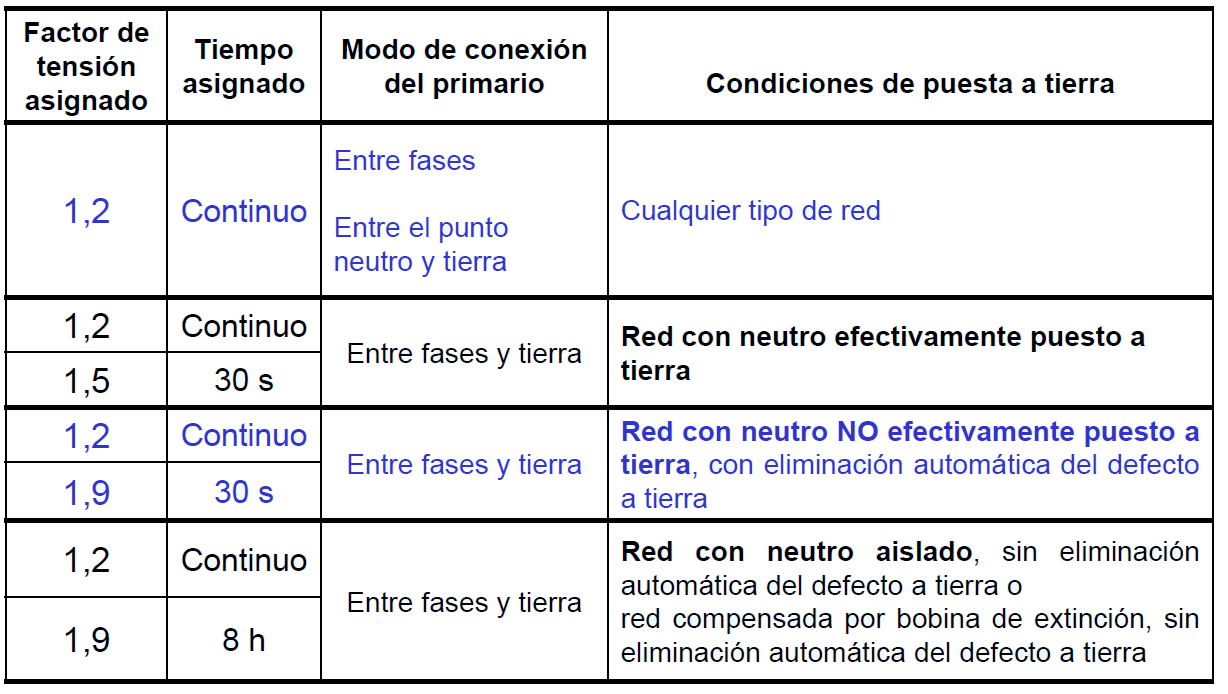
\includegraphics[width=0.7\linewidth]{Images/50}
			\label{fig:50}
		\end{figure}
		
		
		
		\item \textbf{Clase de precisión TT de protección}:  Valor máximo del error de relación (\%)
		\begin{itemize}
			\item Tensión:entre el 5 \% de la tensión asignada $U_{pn}$ y el factor de tensión asignado
			\item Carga: 25 \% y 100 \% de la carga de precisión
			\item fdp = 0,8 inductivo
		\end{itemize}
		Al 2 \% de la tensión asignada, los errores límites de tensión y fase pueden ser hasta el doble, de los considerados entre el 5 \% de la tensión asignada y el factor de tensión asignado.

		\begin{table}[H]
			\centering
			\begin{tabular}{|p{5cm}|p{1cm}|p{1cm}|p{1cm}|p{1cm}|p{1cm}|p{1cm}|p{1cm}|p{1cm}|}
				\hline
				\textbf{Clase de precisión} & \multicolumn{4}{p{4cm}|}{\centering \textbf{Error de tensión en \% de la tensión asignada $\varepsilon_u$ (relación) $\pm$}} & \multicolumn{4}{p{4cm}|}{\centering \textbf{Desfase $\varphi_u \pm$} en centiradianes} \\ \hline
				\textbf{Valores de tensión expresados en \% de la tensión asignada} & \textbf{2} & \textbf{5} & \textbf{100} & \textbf{X} & \textbf{2} & \textbf{5} & \textbf{100} & \textbf{X} \\ \hline
				\textbf{3P} & 6,0 & 3,0 & 3,0 & 3,0 & 240 & 120 & 120 & 120 \\ \hline
				\textbf{6P} & 12,0 & 6,0 & 6,0 & 6,0 & 480 & 240 & 240 & 240 \\ \hline
			\end{tabular}
			\label{tab:errores_tension}
		\end{table}
		\begin{table}[H]
			\centering
			\begin{tabular}{|p{4cm}|p{10cm}|}
				\hline
				\textbf{Clase de precisión} & \textbf{Usos más generalizados} \\ \hline
				\textbf{3P} & Relés que exigen cierta precisión y no excesivo error de ángulo (direccionales y de distancia) \\ \hline
				\textbf{6P} & Relés de sobretensión o de mínima tensión, sin requerimientos especiales en cuanto a error de ángulo \\ \hline
			\end{tabular}
			\label{tab:usos_precision}
		\end{table}
	\end{itemize}
\end{itemize}
\subsection{Esquemas de conexión}
Normalmente se conectan entre fase y tierra. A partir de 72.5kV son todos de fase-tierra. Si se conecta entre fases solo se necesitan dos TT para medir las tres tensiones compuestas (solo usado en MT). Se pueden usar trafos con tomas intermedias para equipos auxiliares (da-dn) mientras que en medida (a-n).
\begin{figure}[H]
	\centering
	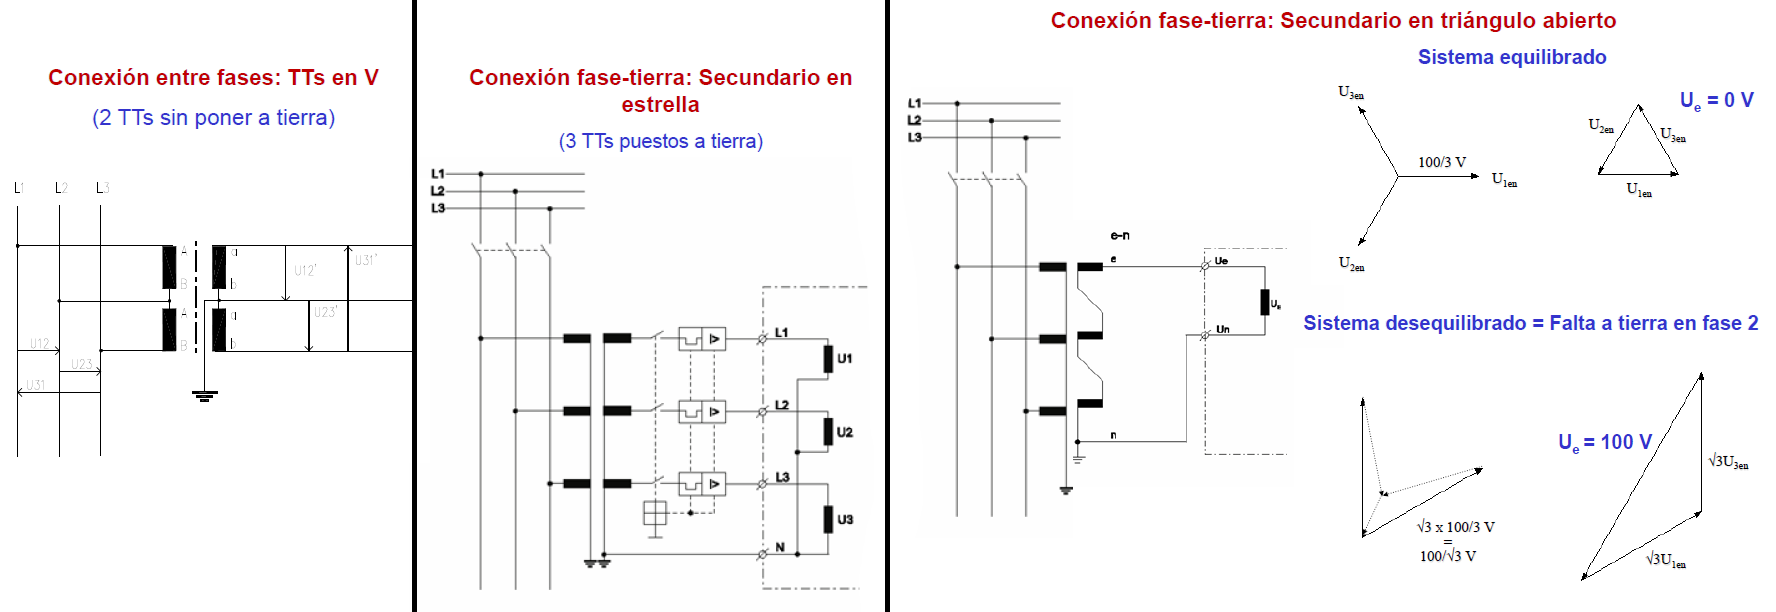
\includegraphics[width=1\linewidth]{Images/51}
	\label{fig:51}
\end{figure}

\section{Transformadores de mínima potencia}
\subsection{Principio de funcionamiento}
Trafos de intensidad:
\begin{itemize}
	\item Transformadores ópticos que utilizan el efecto Faraday
	(cambios del ángulo de polarización de la luz cuando atraviesa un campo magnético)
	\item Transformadores convencionales con salida óptica
	\item Transformadores que utilizan efecto Rogowsky(el voltaje inducido en la bobina es proporcional a la velocidad con la que varía la corriente)
\end{itemize}
Trafos de tensión:
\begin{itemize}
	\item Divisor capacitivo y salida óptica
	\item Efecto Pockels(cambios del ángulo de polarización de la luz cuando atraviesa un campo eléctrico)
\end{itemize}
\subsection{Ventajas}
\begin{itemize}
	\item Transformador de medida y protección comunes
	\item Intensidades secundarias o tensiones más fáciles de procesar, no hay saturación
	\item Mayor seguridad
	\item Gran área de transferencia
	\item Diseño más compacto
	\item Menor variedad de modelos
	\item Ausencia de dieléctricos contaminantes
\end{itemize}